\subsection*{Theorems about Inverse Functions}
The next two results in this section are two important theorems about inverse functions.  The first is actually a corollary of Theorem~\ref{T:inversenotation}.

\begin{corollary} \label{C:inversecomposition}
Let  $A$  and  $B$  be nonempty sets and let  $f\x A \to B$  be a bijection.  Then
\begin{enumerate}
\item For every $x$ in $A$, $\left( f^{ - 1}  \circ f \right)(x) = x$.
\label{C:inversecomposition1}
\item For every $y$ in $B$, $\left( f \circ f^{ - 1}\right)(y) = y$.
\label{C:inversecomposition2}
\end{enumerate}
%\[
%f^{ - 1}  \circ f = I_A \text{  and  } f \circ f^{ - 1}  = I_B 
%\]
%where  $I_A $ is the identity function on  $A$, and  $I_B $ is the identity function on  $B$.
\end{corollary}
%
\begin{myproof}
Let  $A$  and  $B$  be nonempty sets and assume that  $f\x A \to B$  is a bijection. 
%Recall that for every  $x \in A$,  $I_A ( x ) = x$.  
So let  $x \in A$ and let  $f( x ) = y$.  By Theorem~\ref{T:inversenotation}, we can conclude that  $f^{ - 1} ( y ) = x$.  Therefore,
\[
\begin{aligned}
  \left( {f^{ - 1}  \circ f} \right)( x ) &= f^{ - 1} \! \left( {f( x )} \right) \\ 
                                          &= f^{-1}( y ) \\ 
                                          &= x. \\ 
\end{aligned}
\] 
Hence, for each  $x \in A$, $\left( {f^{ - 1}  \circ f} \right)( x ) = x$.

The proof that for each $y$ in $B$, $\left( f \circ f^{ - 1}\right)(y)  = y$ is 
Exercise~(\ref{exer:inversecomposition}).
\end{myproof}
%\hbreak
%
\addtocounter{theorem}{-2}
\begin{example}[\textbf{continued}] \hfill \\
For the cubing function and the cube root function, we have seen that
\begin{center}
For  $x, y \in \R$,  $x^3  = y$  if and only if  $\sqrt[3]{y} = x$.
\end{center}
Notice that
\begin{itemize}
\item If we substitute  $x^3  = y$ into the equation  $\sqrt[3]{y} = x$, we obtain
$\sqrt[3]{{x^3 }} = x$.

\item If we substitute  $\sqrt[3]{y} = x$ into the equation  $x^3  = y$, we obtain 
$\left( {\sqrt[3]{y}} \right)^3  = y$.
\end{itemize}
This is an illustration of Corollary~\ref{C:inversecomposition}.  We can see this by using 
$f\x \R \to \R$  defined by  $f( x ) = x^3 $ and   
$f^{ - 1} \x \R \to \R$  defined by  $f^{ - 1} ( y ) = \sqrt[3]{y}$.   Then  
$f^{ - 1}  \circ f\x \R \to \R$ and $f^{ - 1}  \circ f = I_\R $.  So for each $x \in \R$,
\[
\begin{aligned}
  \left( {f^{ - 1}  \circ f} \right)( x ) &= x \\ 
      f^{ - 1} \! \left( {f( x )} \right) &= x \\ 
         f^{ - 1} \!\left( {x^3 } \right) &= x \\ 
                         \sqrt[3]{{x^3 }} &= x. \\ 
\end{aligned}
\]
Similarly, the equation  $\left( {\sqrt[3]{y}} \right)^3  = y$ for each  $y \in \R$ can be obtained from the fact that for each $y \in \R$,  $(f \circ f^{ - 1})(y) = y$.
\end{example}
\hbreak
%
\addtocounter{theorem}{1}
%

We will now consider the case where  $f\x A \to B$  and  $g\x B \to C$  are both bijections.   In this case,  $f^{ - 1} \x B \to A$  and  $g^{ - 1} \x C \to B$.  
Figure~\ref {fig:bijectioncomposition} can be used to illustrate this situation.
\begin{figure}[h]
\begin{center}
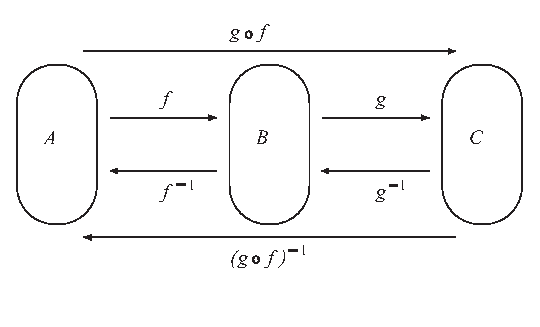
\includegraphics{figps-compinverse.eps}
\caption{Composition of Two Bijections} \label{fig:bijectioncomposition}
\end{center}
\end{figure}

%
By Theorem~\ref{T:compositefunctions},  $g \circ f\x A \to C$  is also a bijection. Hence, by Theorem~\ref{T:inverseandbijection},  
$( {g \circ f} )^{ - 1} $ is a function and, in fact, 
$( {g \circ f} )^{ - 1} \x C \to A$.  Notice that we can also form the composition of  $g^{ - 1} $  followed by  $f^{ - 1} $ to get  $f^{ - 1}  \circ g^{ - 1} \x C \to A$.  Figure~\ref {fig:bijectioncomposition} helps illustrate the result of the next theorem.
%
\setcounter{equation}{0}
\begin{theorem} \label{compositionofbijections}
Let $f\x A \to B$  and  $g\x B \to C$  be bijections.  Then  $g \circ f$  is a bijection and  
$( {g \circ f} )^{ - 1}  = f^{ - 1}  \circ g^{ - 1} $.
\end{theorem}
%
\begin{myproof}
Let $f\x A \to B$  and  $g\x B \to C$  be bijections.  Then  $f^{ - 1} \x B \to A$  and  
$g^{ - 1} \x C \to B$.  Hence, $f^{ - 1}  \circ g^{ - 1} \x C \to A$.  Also, by Theorem~\ref{T:compositefunctions},  $g \circ f\x A \to C$  is a bijection, and hence 
$( {g \circ f} )^{ - 1} \x C \to A$.   We will now prove that for each  
$z \in C$, 
$( {g \circ f} )^{ - 1} ( z ) = ( {f^{ - 1}  \circ g^{ - 1} } )( z )$.

Let  $z \in C$.  Since the function  $g$  is a surjection, there exists a  $y \in B$ such that
\begin{equation} \label{eq:compofbij1} 
g( y ) = z.
\end{equation}
%
Also, since  $f$  is a surjection, there exists an  $x \in A$  such that
\begin{equation} \label{eq:compofbij2}
f( x ) = y.
\end{equation}
%
Now these two equations can be written in terms of the  respective inverse functions as
\begin{align}
g^{ - 1} ( z ) &= y; \text{ and }  \label{eq:compofbij3}\\
f^{ - 1} ( y ) &= x.  \label{eq:compofbij4}
\end{align}
%
Using equations~(\ref{eq:compofbij3}) and~(\ref{eq:compofbij4}), we see that
\begin{align}  \notag
  \left( {f^{ - 1}  \circ g^{ - 1} } \right)( z ) &= f^{ - 1} \left( {g^{ - 1} ( z )} \right) \\ \notag
                                                  &= f^{ - 1} ( y ) \\ \label{eq:compofbij5}                                                  &= x. \\  \notag
\end{align} 
%
Using equations~(\ref{eq:compofbij1}) and~(\ref{eq:compofbij2})  again, we see that  
$( {g \circ f} )( x ) = z$.  However, in terms of the inverse function, this means that
\begin{equation} \label{eq:compofbij6}
( {g \circ f} )^{ - 1} ( z ) = x.
\end{equation}
%
Comparing equations~(\ref{eq:compofbij5}) and~(\ref{eq:compofbij6}), we have shown that for all  $z \in C$,
\linebreak 
$( {g \circ f} )^{ - 1} ( z ) = ( {f^{ - 1}  \circ g^{ - 1} } )( z )$.  This proves that  
$( {g \circ f} )^{ - 1}  = f^{ - 1}  \circ g^{ - 1} $.
\end{myproof}
\hbreak

\endinput
